\documentclass{beamer}
%
% Choose how your presentation looks.
%
% For more themes, color themes and font themes, see:
% http://deic.uab.es/~iblanes/beamer_gallery/index_by_theme.html
%
\usetheme[style=simple,nat]{Frederiksberg}
\usefonttheme{serif}  

\usepackage{Nikolai}
\usepackage[english]{babel}
\usepackage[super]{nth}


\title{Visualisation of Concepts in Condensed Matter Physics}
\author{Nikolai Plambech Nielsen}
\institute{Niels Bohr Institute}
\date{\nth{27} of June, 2018}

\begin{document}

\begin{frame}
  \titlepage
\end{frame}


\section{Outline}
\begin{frame}{Outline}
\begin{itemize}
  \item Introduction
  \item Background
  \item Lattices and crystal structure
  \item The reciprocal lattice and scattering
  \item Band structure
\end{itemize}
\end{frame}



\section{Introduction}
\begin{frame}{Introduction}
\end{frame}


\section{Background}
\begin{frame}{Background}
Bloch's theorem
\begin{equation*}
	\psi(\V{r}) = e^{i \V{k}\D \V{r}} u(\V{r}) = \sum_{\V{G}} u_{\V{G},\V{k}} e^{i (\V{G}+\V{k}) \D \V{r}}
\end{equation*}
\end{frame}


\section{Lattices and crystal structure}
\begin{frame}{Lattices and crystal structure}
\begin{equation*}
	\V{R} = \sum_{i = 1}^{d} n_i \V{a}_i
\end{equation*}
\begin{figure}[H]
	\centering
	\begin{minipage}{.4\textwidth}
		\centering
		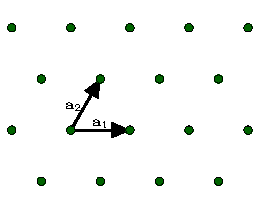
\includegraphics[width=\linewidth]{figures/triangular.pdf}
		\captionof{figure}{A triangular lattice. $ \V{a}_1 = a\D(1,0)$, \\$\V{a}_2 = a\D(1/2, \sqrt{3}/2) $}
		\label{fig:triangular_lattice}
	\end{minipage}%
	\hfill
	\begin{minipage}{.4\textwidth}
		\centering
		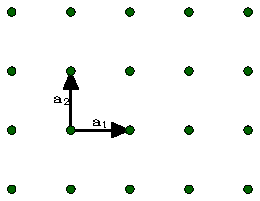
\includegraphics[width=\linewidth]{figures/square.pdf}
		\captionof{figure}{A square lattice. $ \V{a}_1 = a\D(1,0), \V{a}_2 = a\D(0,1) $}
		\label{fig:square_lattice}
	\end{minipage}
\end{figure}
\end{frame}


\begin{frame}{Lattices and crystal structure}
\begin{equation*}
\V{R} = \sum_{i = 1}^{d} n_i \V{a}_i
\end{equation*}
\begin{figure}[H]
	\centering
	\begin{minipage}{.4\textwidth}
		\centering
		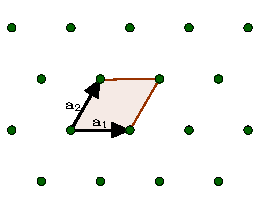
\includegraphics[width=\linewidth]{figures/triangularUnit.pdf}
		\captionof{figure}{A triangular lattice. $ \V{a}_1 = a\D(1,0)$, \\$\V{a}_2 = a\D(1/2, \sqrt{3}/2) $}
		\label{fig:triangular_unitcell}
	\end{minipage}%
	\hfill
	\begin{minipage}{.4\textwidth}
		\centering
		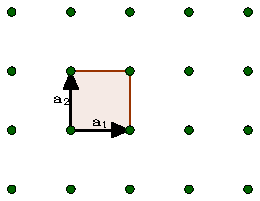
\includegraphics[width=\linewidth]{figures/squareUnit.pdf}
		\captionof{figure}{A square lattice. $ \V{a}_1 = a\D(1,0), \V{a}_2 = a\D(0,1) $}
		\label{fig:square_unitcell}
	\end{minipage}
\end{figure}
\end{frame}


\begin{frame}{Lattices and crystal structure}
\begin{equation*}\label{key}
	\V{r}_{atom,i} = \V{R} + \V{r}_{basis, i}
\end{equation*}
\begin{figure}[H]
	\centering
	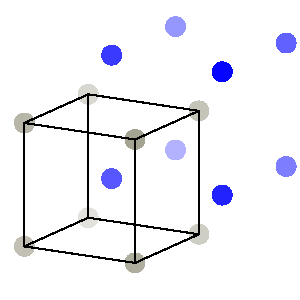
\includegraphics{figures/lattice_unfinished_1.pdf}
	\caption{Conventional unit cell of a bcc lattice. Two atoms, one (grey) at $ a \D (0,0,0) $ and one (blue) at $ a\D(1/2, 1/2, 1/2) $}
\end{figure}
\end{frame}


\begin{frame}{Lattices and crystal structure}
\end{frame}



\section{Reciprocal lattice and scattering}
\begin{frame}{Reciprocal lattice and scattering}
\begin{equation*}
	e^{i \V{G} \D\V{R}} = 1,
\end{equation*}
\begin{equation*}\label{key}
	\V{G} = m_1 \V{b}_1 + m_2 \V{b}_2 + m_3\V{b}_3, \quad \V{a}_i \D \V{b}_j = 2\pi \delta_{ij}
\end{equation*}
\begin{align*}\label{key}
	\V{b}_1 &= \frac{2\pi \, \V{a}_2 \times \V{a}_3}{\V{a}_1 \D (\V{a}_2 \times \V{a}_3)}, \quad \V{b}_2 = \frac{2\pi \, \V{a}_3 \times \V{a}_1}{\V{a}_2 \D (\V{a}_3 \times \V{a}_1)}, \\
	\V{b}_3 &= \frac{2\pi \, \V{a}_1 \times \V{a}_2}{\V{a}_3 \D (\V{a}_1 \times \V{a}_2)},
\end{align*}
\end{frame}


\begin{frame}
Fermi's Golden Rule
\begin{equation}\label{key}
	\Gamma(\V{k}', \V{k}) = \frac{2\pi}{\hbar}|\braket{\V{k}' | V | \V{k}}|^2 \delta(E_{\V{k}'}-E_{\V{k}}),
\end{equation}
\end{frame}
\end{document}
